\documentclass[11pt,a4paper,DIV=14,headinclude=false,footinclude=false]{scrartcl}
\usepackage[utf8]{inputenc}
%!TeX spellcheck = en_GB
\usepackage[english]{babel}
\usepackage[T1]{fontenc}
\usepackage{lmodern}

\usepackage{enumitem} % Extended enumerate: label= ...
\usepackage{listings} % Code formatting
% Math
%\usepackage{amsmath}
\usepackage{mathtools} % amsmath extension
\usepackage{amsfonts} % Math fonts
\usepackage{amssymb}
%\usepackage{amsthm} % Theorems, like proof
%\usepackage{stmaryrd} % More symbols, like \lightning, rrbracket, ...
% Tables
\usepackage{array} % Extended options for array and tabular
\usepackage{booktabs} % Rules for tables
%\usepackage{tabu} % Extended table environment
% Graphics and floats
\usepackage{graphicx}
%\usepackage{placeins} % \FloatBarrier
\usepackage{float} % [H] for floats
% Refs
\usepackage[bookmarks=true,bookmarksnumbered=true,colorlinks=false,linkbordercolor={0 0 0},pdfborder={0 0 0}]{hyperref}
%\usepackage[all]{hypcap} % Link to top of figure and table
\usepackage{caption}
\usepackage{lastpage}

% Style
\setkomafont{captionlabel}{\bfseries}
%\setcounter{secnumdepth}{-1} % Disables chapter and section numbering
%% Margins
%%\usepackage[top=2.5cm,head=2.5cm,headsep=0.5cm,inner=2cm,outer=2cm,bottom=2.5cm,footskip=1cm]{geometry}
%% Header and footer
\usepackage{scrlayer-scrpage}
\clearpairofpagestyles
\setkomafont{pageheadfoot}{\normalfont\sffamily}
%\pagestyle{scrheadings}
%%\setheadsepline{}[\ifthispageodd{}{\setheadsepline{0pt}}] % No headsepline for even pages
%%========================%
%\lohead{\small\begin{tabular}{@{}l@{ }l}
%    Ralph Lesch
%\end{tabular}
%}
%\cohead{\bfseries Deep Learning Lab WS2018 -- Exercise 3}
%\rohead{2018-12-04}
%%
\cfoot[\pagemark/\pageref{LastPage}]{\pagemark/\pageref{LastPage}} % Site number

\begin{document}
\title{Deep Learning Lab WS2018\\Exercise 4 -- CV/ML}
\author{Ralph Lesch}
\maketitle

\noindent In this exercise we combine Bayesian Optimization (BO) with Hyperband (HB) in three steps:
\begin{enumerate}
\item Implementing Bayesian Optimization using emukit.
\item Hyperband with its successive halving
\item Combination of Bayesian optimization with Hyperband (BOHB)
\end{enumerate}
To reduce compilation time, we use a surrogate benchmark, a regression model (random forest) of the original benchmark (CNNs).
\section{Bayesian Optimization}\label{sec:BO}
Operating on the surrogate benchmark, the Bayesian Optimization with emukit using ExpectedImprovement on a Gaussian process as a probabilistic model gives clear optimization steps, as shown in \autoref{fig:BO}. Samples are generated using emukit's RandomDesign.
\begin{figure}[hb]\centering
	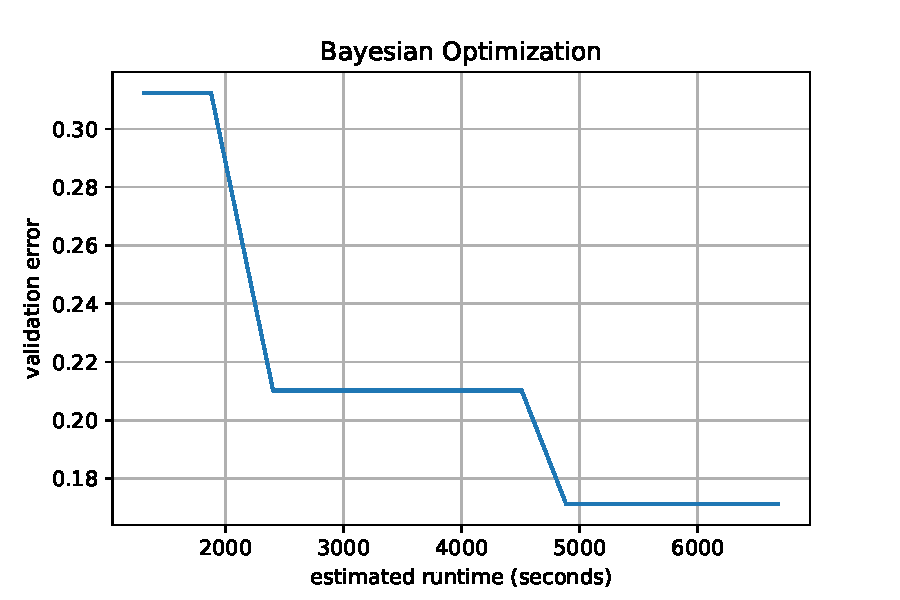
\includegraphics[width=.6\linewidth]{plots/BO.pdf}
	\caption{Bayesian Optimization}\label{fig:BO}
\end{figure}

\section{Hyperband}
For Hyperband, we use the same uniform random sample generation, as with \hyperref[sec:BO]{BO}. The results of the successive halving are shown in \autoref{fig:HB}.

\begin{figure}[h]\centering
    \newcommand\trimmedgraphics[2][]{\includegraphics[width=\linewidth,keepaspectratio,clip,trim=0 0 30px 31px,#1]{#2}}
    \begin{minipage}{.5\textwidth} \centering
        1. successive halving (s=3)
        \trimmedgraphics{plots/HB_s=3.pdf}
%        \caption{config 1}
    \end{minipage}\hfill
    \begin{minipage}{.5\textwidth}\centering
        2.  (s=2)
        \trimmedgraphics{plots/HB_s=2.pdf}
%        \caption{config 2}
     \end{minipage}\\[\baselineskip]
%\end{figure}
%\begin{figure}[hbt]\centering
    \begin{minipage}{.5\textwidth} \centering
        3. (s=1)
        \trimmedgraphics{plots/HB_s=1.pdf}
%        \caption{config 3}
    \end{minipage}\hfill
    \begin{minipage}{.5\textwidth}\centering
        4. (s=0)
        \trimmedgraphics{plots/HB_s=0.pdf}
%        \caption{config 4}
     \end{minipage}
     \caption{Hyperband: successive halving}\label{fig:HB}
\end{figure}
\section{Bayesian Optimization with Hyperband}
You can see in \autoref{fig:BOHB}, how the sampling from the implemented model with the combination BOHB gives in average a smaller validation error than the random sampled configuration, as expected.
\begin{figure}[H]\centering
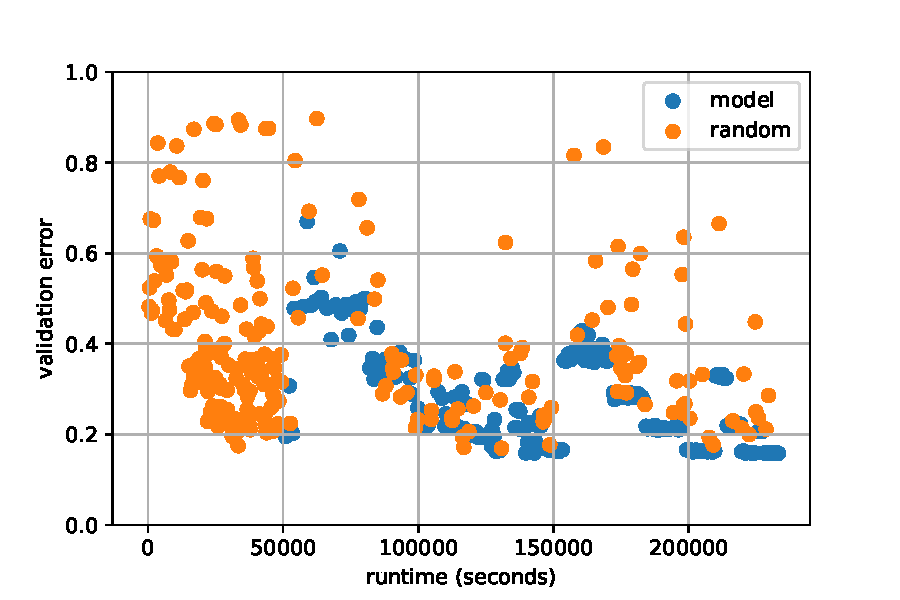
\includegraphics[width=0.6\linewidth]{plots/BOHB.pdf}
\caption{BOHB vs random sampled}\label{fig:BOHB}
\end{figure}

\end{document}
